%%%%%%%%%%%%%%%%%%%%%%%%%%%%%%%%%%%%%%%%%%%%%%%%%%%%%%%%%%%%%%%%%%%%%%%%%%%%%%%%%%%%%%%%%
% Section 10: Installing New Devices
%	This section provides a detailed walkthrough on how to install new devices
%	to be used in RapidSmith.
%%%%%%%%%%%%%%%%%%%%%%%%%%%%%%%%%%%%%%%%%%%%%%%%%%%%%%%%%%%%%%%%%%%%%%%%%%%%%%%%%%%%%%%%%
\newpage
\section{Installing New Device Files} \label{sec:installingDeviceFiles}
The device files included with the RapidSmith2 installation (listed in
\autoref{sec:supportedDevices}) have been well-tested, and are great starting
points for new users. If you are a new user, it is \emph{strongly encouraged}
that you learn RapidSmith's APIs and data structures by first implementing CAD tools on
these devices. However, RapidSmith2 also supports installing new device files
for parts not listed in \autoref{sec:supportedDevices}. This section contains
the following: (1) a description of the required intermediate files that need to be
generated from \texttt{Tincr} to support a new device, and (2) the necessary
steps to transform the intermediate files into compact device files that can be
loaded into RapidSmith2.

\subsection {XDLRC}
The \texttt{Device} data structures in RapidSmith are mainly created from XDLRC
files. XDLRC files contain a complete physical description of a Xilinx device
(including tiles, wires, sites, etc.). For older Xilinx parts (series 7 and
below), these files can be created in ISE with the \texttt{xdl} command. For
newer parts (UltraScale and above), XDLRC files can be created in Vivado using
the \texttt{Tincr} command \textit{tincr::write xdlrc}. Because XDLRC files can
grow to be hundreds of Gigabytes in size, RapidSmith compresses them into much smaller device files
(usually in the tens of Megabytes). \autoref{sec:appendixXDLRC} contains a more
detailed description of XDLRC syntax for those who are interested.

\subsection{FamilyInfo}
A \textit{familyInfo.xml} file contains useful information that is
not included in the XDLRC files for a given family of devices. Vivado currently 
supports 8 different family types: Artix7, Virtex7, Kintex7, Zynq, Kintex
UltraScale, Virtex UltraScale, Kintex UltraScale+, and Virtex UltraScale+. Only
one \textit{familyInfo.xml} file is required for each of these families (all 
devices within a family share the same family info). The remainder of this
section describes the important parts of a \textit{familyInfo.xml} file, and how
they are represented in RapidSmith2.

\begin{itemize}
  \item A list of \textbf{compatible types} for each site. Site A is said to be
  compatible with site B if the logical cells placed on site A can
  \textit{always} be placed on site B as well. For example, as shown in
  \autoref{fig:sliceCompatibility}, SLICEL sites are compatible with SLICEM
  sites. The cells placed on the SLICEL in the figure can be moved to the
  SLICEM and function indentically. SLICEM sites, however, are \textit{not}
  compatible with SLICEL sites. This is because SLICEM sites support LUT RAM
  cells, which cannot be placed on SLICEL sites.
  
  \begin{figure}[H]
    \centering
    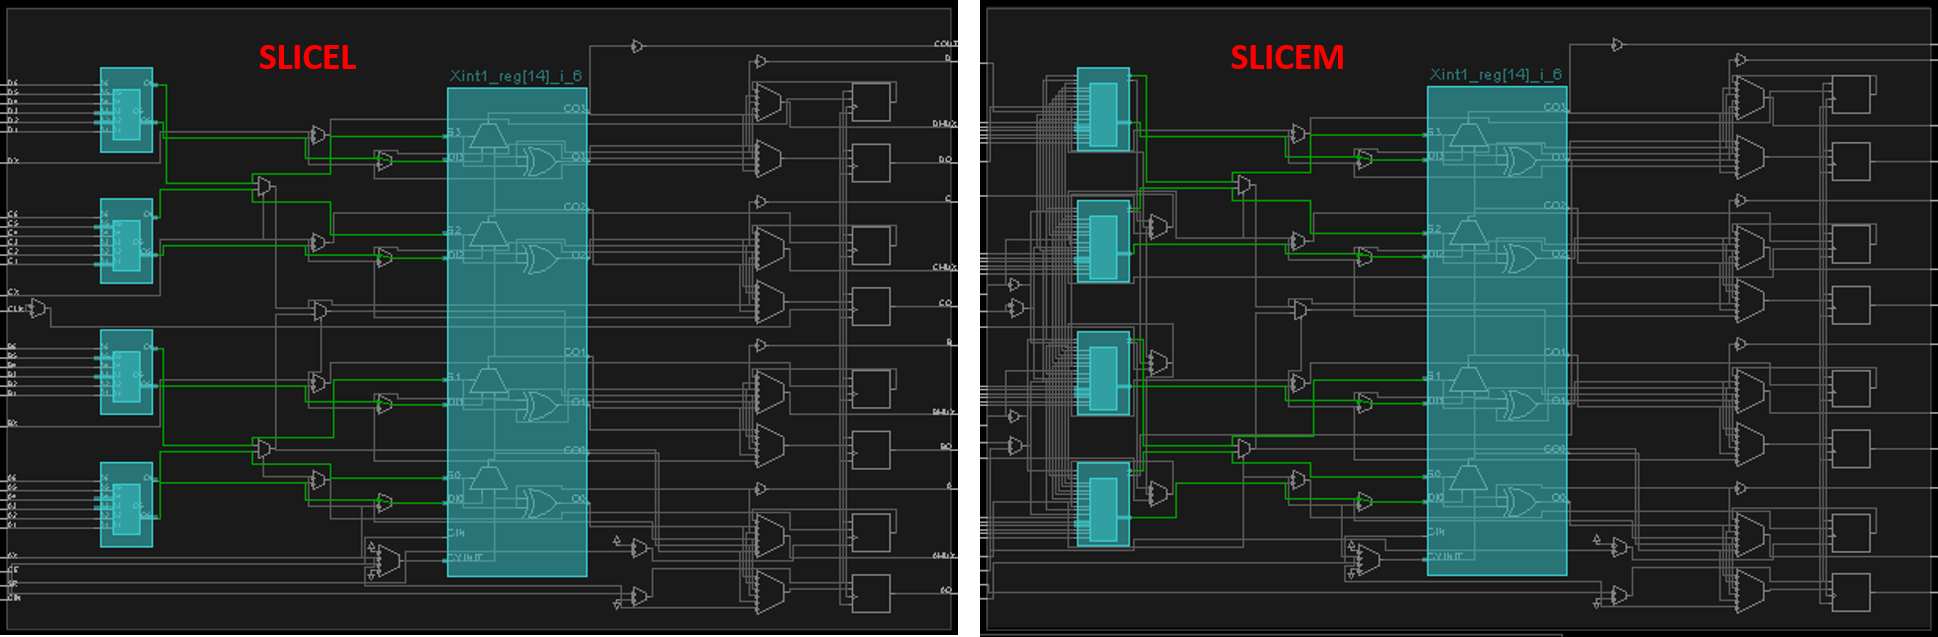
\includegraphics[width=1\columnwidth]{compatibleSites.png}
    \caption{The same group of cells placed on a SLICEL site (left) and a SLICEM
    site (right).}
    \label{fig:sliceCompatibility}
  \end{figure}
  
  \noindent Compatible sites are important
  to site-level placers in determining where a group of cells can be placed.
  \textbf{NOTE}: In some instances of compatibility, you have to first change
  the type of the compatible site before placing cells on it. For example, a
  RAMB36 site is compatible with a RAMBFIFO36 site. However, the site type of
  the RAMBFIFO36 site \textbf{must be changed to a RAMB36} before it is
  truly compatible.
  
  \item A list of \textbf{routethrough connections} for each LUT BEL (including
  the input bel-pin and output bel-pin of the routethrough). These routethrough
  connections are turned into \texttt{Connection} objects in RapidSmith2 that
  can be used for internal site routing. Sections \ref{sec:routing} and
  \ref{sec:additionalInfo} give more information about LUT routethroughs.
  
  \item A list of \textbf{alternate types} for each site. Each physical site on
  the device has an associated default type. Some sites, however, can be
  configured to be one of many types. An example for an UltraScale
  BITSLICE\_RX\_TX site is shown in \autoref{fig:alternateTypes}. As the figure
  shows, a BITSLICE\_RX\_TX site can also be configured to be of type
  BITSLICE\_COMPONENT\_RX\_TX, BITSLICE\_RXTX\_RX, or BITSLICE\_RXTX\_TX.
  RapidSmith2 parses the alternate site information from the XML and applies it
  to the corresponding \texttt{Site} data structure. This allows users to change
  site types based on what they need.
  
  \begin{figure}[H]
    \centering
    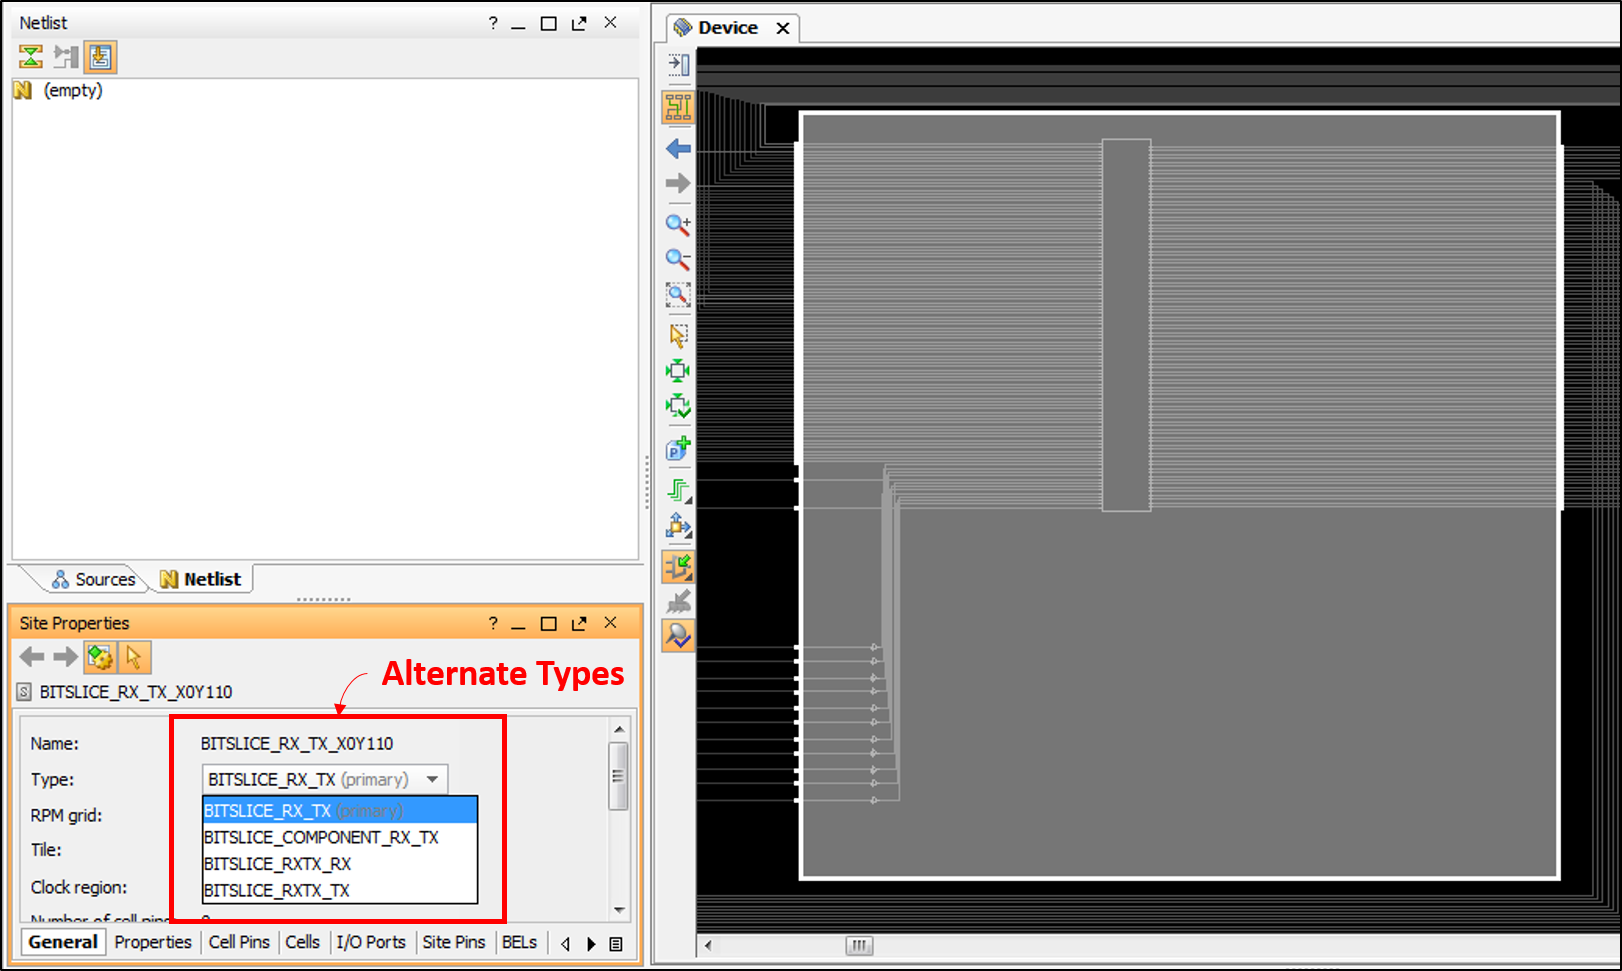
\includegraphics[width=.8\columnwidth]{alternateTypes.png}
    \caption{Vivado GUI showing alternate types for a BITSLICE\_RX\_TX site.}
    \label{fig:alternateTypes}
  \end{figure}
  
  \item A list of \textbf{site pip corrections}. In the XDLRC files that are
  parsed into RapidSmith, site pips (or routing muxes) are not distinguished
  from the functional BELs (such as LUTs and Flip Flops) of a site. The
  Family Info XML identifies the site pips of a site and marks them as either
  a ``mux'' or a ``polarity\_selector.'' RapidSmith2 transforms these routing
  muxes into individual pips as shown in \autoref{fig:sitePipDecomposition} so
  that they are no longer represented as BELs. After the decomposition, each pip
  is a routing resource of the site.
  
  \begin{figure}[H]
    \centering
    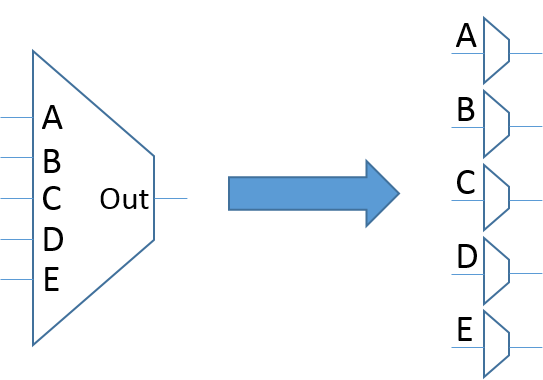
\includegraphics[width=.5\columnwidth]{sitePipDecomposition.png}
    \caption{RapidSmith2 site pip decomposition.}
    \label{fig:sitePipDecomposition}
  \end{figure}
  
  \item A list of \textbf{pin direction corrections}. For ISE-generated XDLRC
  files, all bel-pins are given a direction of either INPUT or OUTPUT. However,
  there are several bel-pins in Xilinx devices that are actually of direction
  INOUT (bidirectional). The Family Info file marks INOUT bel-pins so that
  their direction can be corrected in RapidSmith2.
  
\end{itemize}

\subsection{Creating New Device Files for Supported Families} \label{sec:creatingNewSupportedDevices} 
Subsection \ref{sec:supportedDevices} gives a list of currently supported
families in RapidSmith2. If the device you want to install is \textbf{not} within a
supported family, see \autoref{sec:newFamilies} for how to add support for a
new family in RapidSmith. Otherwise, a new device file can be added in two easy
steps:

\begin {enumerate}
\item Open Vivado in Tcl mode, and execute the \texttt{Tincr} command
\textit{::tincr::write\_xdlrc}. An example command usage is given below for the
Artix7 part \textit{xc7a100tcsg324-3}.

\begin{lstlisting}[numbers=none]
[ttown523@CB461-EE09968:�] vivado -mode tcl

****** Vivado v2014.2 (64-bit)
 **** SW Build 928826 on Thu Jun 5 17:55:10 MDT 2014
 **** IP Build 924643 on Fri May 30 09:20:16 MDT 2014
  ** Copyright 1986-2014 Xilinx, Inc. All Rights Reserved.

Vivado% ::tincr::write_xdlrc -part xc7a100tcsg324-3 -max_processes 4 -primitive_defs xc7a100tcsg324_full.xdlrc
\end{lstlisting}

\noindent The ``-max\_processes'' option is used to parallelize the operation so
that it will execute faster. If you have problems with the parallel generation
however (it can sometimes hang), then setting this option to ``1'' will
prevent the process from hanging. \textbf{NOTE}: This Tcl command can take a
very long time to run (more than 24 hours for very large devices). It is
suggested that you run it on a remote machine so that you can continue work on
your regular work machine. Also, be aware that these XDLRC files are massive. 100 GB
for the largest XDLRC files is not uncommon. Make sure you have enough space on
your hard drive before generating the XDLRC for a device.

\item Run the device installer in RapidSmith2 and pass the newly created XDLRC
as an argument. An example command line usage is shown below. The device
installer can also be run in an IDE.

\begin{lstlisting}[numbers=none]
[ttown523@CB461-EE09968:�] java -ea -Xmx4096m edu.byu.ece.rapidSmith.util.Installer --generate file xc7a100tcsg324_full.xdlrc
\end{lstlisting} 

\noindent The device installer parses the verbose XDLRC file, and creates
compact RapidSmith device files (Megabytes instead of Gigabytes) that represent
a Xilinx device. Notice the two JVM command line arguments used in the command
above. The first option (``-ea'') enables assertions for the code. It is important
to include this flag so that device file errors can be caught during parsing.
If you are creating a new device file for a supported family however, there
should be no errors during the installation process. The second option
(``-Xmx4096m'') sets how much memory the JVM can use while running the
installer. Since XDLRC files are so large, the memory usage of the installer can
grow very quickly. In the command above, the JVM is set to use 4 GB of memory.
If the device installer fails with an out of memory exception, you will
need to increase the number of this parameter and re-run the installer (you may
need up to 32 GB of memory here). Once the device installer is done executing,
the compact devices files are stored in the corresponding family directory of
the RapidSmith2 ``devices'' folder. For example, the device files generated
from the example part \textit{xc7a100tcsg324-3} are stored in the ``artix7''
sub-directory. The listing below shows the two device files that are created
after the device installer has completed (the device files are bolded).

\begin{lstlisting}[numbers=none]
[ttown523@CB461-EE09968:artix7] ls
cellLibrary.xml familyInfo.xml |\textbf{xc7a100tcsg324\_db.dat}| |\textbf{xc7a100tcsg324\_info.dat}|
\end{lstlisting} 

\noindent  The file ending in ``\_db.dat''
contains the serialized \texttt{Device} data structures for RapidSmith. The file
ending in ``\_info.dat'' contains additional serialized data (such as reverse
wire connections) that can be optionally loaded with the device.

\item Run the Family Builder in RapidSmith2 and pass your part as the command
line argument. An example usage is shown below for an Artix7 device.

\begin{lstlisting}[numbers=none]
[ttown523@CB461-EE09968:�] java edu.byu.ece.rapidSmith.util.FamilyBuilders xc7a100tcsg324
\end{lstlisting}

\noindent An Artix7.java (or whatever family your device is in) will already
exist, but will be updated with new sites and tile types from your newly
installed part.
\end{enumerate}

\noindent After running these steps, the part is ready to be used in RapidSmith.
See \autoref{sec:loadingDevice} for how to load the device and begin using it.

\subsection{Supporting New Device Families} \label{sec:newFamilies}
Vivado supports implementing FPGA designs on devices for the following families
(also called architectures):

\begin{multicols}{2}
	\begin {itemize}
	  \item \textbf{Artix7 (artix7)}
	  \item Kintex7 (kintex7)
	  \item Virtex7 (virtex7)
	  \item Zynq (zynq)
	  \item \textbf{Kintex Ultrascale (kintexu)}
	  \item Virtex Ultrascale (virtexu)
	  \item Kintex Ultrascale+ (kintexuplus)
	  \item Virtex Ultrascale+ (virtexuplus)
	  \item *Future Devices
	\end{itemize}
\end{multicols}

\noindent The name in parentheses is the Vivado Tcl name for the family. Bolded
items are families that are currently supported in RapidSmith2 and
\texttt{Tincr}. To add RapidSmith support for another Vivado family, follow the
steps listed below.

\begin {enumerate}
  \item Create the primitive definitions (also called primitive defs) of the
  family using VSRT. As described in \autoref{sec:appendixXDLRC}, the primitive
  definition section of an XDLRC file defines the internal components and
  configuration options of each primitive site in a device. Due to Vivado Tcl
  limations, a complete set of primitive defs cannot be automatically generated from Vivado,
  and some manual work is required. The VSRT user guide 
  {\color{blue}\url{https://github.com/byuccl/RapidSmith2/blob/ultrascale/doc/VSRTUserGuide.pdf}}\\ 
  describes in great detail how to generate a complete set of primitive defs
  for a family of Vivado devices. Follow the guide to create the primitive defs
  for your family. \textbf{NOTE}: Families within the same series (i.e. series
  7, ultrascale, ultrascale+, etc.) share several primitive defs. For example,
  many primitive defs between Kintex UltraScale and Virtex UltraScale families
  are identical. You may be able to reuse existing primitive definitions
  between families. Also, you don't need to generate primitive defs for series7
  devices, they already exist from ISE.
  
  \item Copy the primitive definitions you created in step (1) to the
   directory \textit{tincrPath/cache/family/primitiveDefs}, where ``tincrPath''
   is the path to your \texttt{Tincr} installation and ``family'' is the family
   for the primitive defs you just generated (use the Vivado Tcl name if you
   need to create a new folder).
   
   \item Create the \textit{familyInfo.xml}. To do this, open Vivado in Tcl mode
   and execute the command \\
   \textit{::tincr::create\_xml\_family\_info}. An example usage of the command
   is shown below for Kintex UltraScale. 
   
\begin{lstlisting}[numbers=none]
[ttown523@CB461-EE09968:�] vivado -mode tcl

****** Vivado v2014.2 (64-bit)
 **** SW Build 928826 on Thu Jun 5 17:55:10 MDT 2014
 **** IP Build 924643 on Fri May 30 09:20:16 MDT 2014
  ** Copyright 1986-2014 Xilinx, Inc. All Rights Reserved.

Vivado% ::tincr::create_xml_family_info familyInfo.xml kintexu addedBels.txt 
\end{lstlisting}
	
	\noindent As the listing shows, there are three arguments to the command:
	\begin{itemize}
	  \item \textbf{familyInfo.xml}: The file name to store the generated family
	  info. The file ending ``.xml" will be appended if it is not included.
	  \item \textbf{kintexu}: The Vivado family name.
	  \item \textbf{addedBels.txt} (Optional): When you are generating primitive
	  defs using VSRT (in step 1), a text file called ``addedBels.txt" is created in
	  your VSRT directory. This file contains a list of added VCC/GND BELs for
	  each family. To generate a complete Family Info file, pass this text file as
	  the third argument to the above command. The default argument is an empty
	  string so that no extra BELs will be added to the family info.
	\end{itemize}    
    
    \item Modify the generated Family Info. After step (3) is complete, a few
    hand edits are required to complete the family info file. The required hand
    edits are different between series7 and other devices.
    
    \bigbreak \noindent
	\begin{large}
	\textbf{Series7}
	\end{large}
    
    \noindent Due to complications with Vivado's Tcl interface, there are
    several hand edits that are required to complete the series7 family info
    files. RapidSmith2 already provides support for all series7 families, 
    but the required manual edits are documented here in case they need to
    be regenerated for some reason. 
    
    \begin{enumerate}
      \item The first hand edit is to remove invalid alternate types. For IPAD
      sites, Vivado's Tcl interface reports two alternate site types:
      IOB18M and IOB18S. These site types are not actually valid alternate
      types, meaning they need to be removed. \autoref{fig:ipadAlternates}
      demonstrates the actual alternate types of an IPAD as shown in the Vivado
      GUI.
      
      \begin{figure}[H]
        \centering
        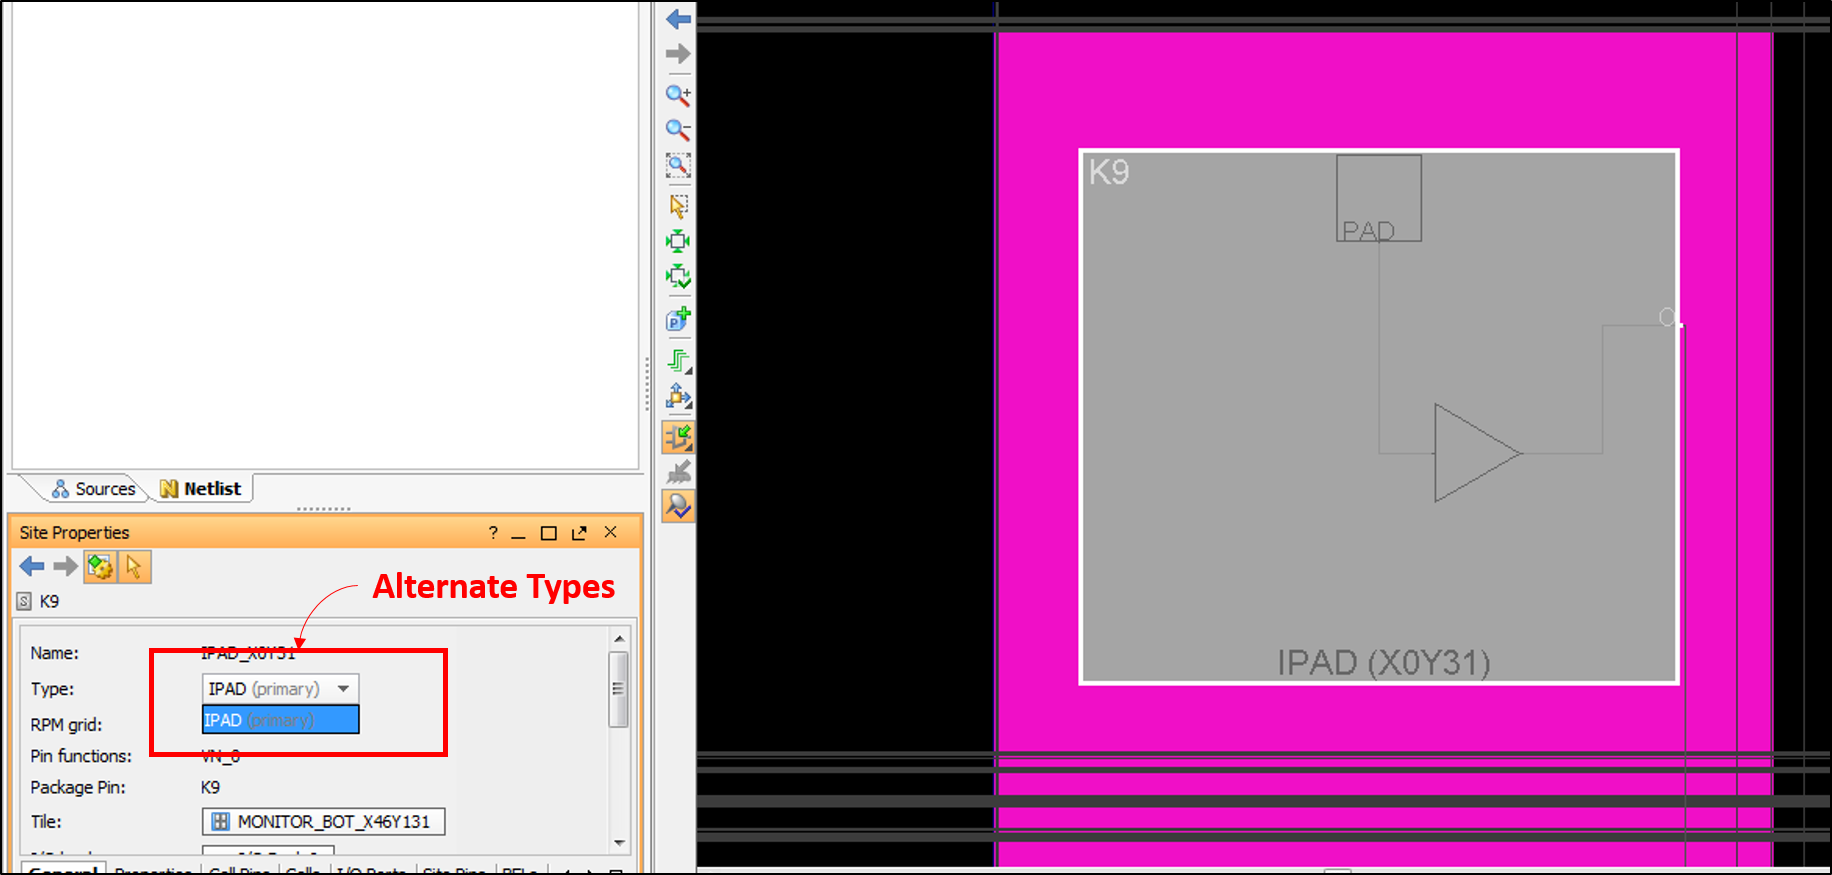
\includegraphics[width=.8\columnwidth]{ipadAlternates.png}
        \caption{Alternate types of an IPAD site (highlighted in red)}
        \label{fig:ipadAlternates}
      \end{figure}
      
      \noindent As the figure shows, there are no valid alternate types.
      The only way to determine invalid alternate types is to go site-by-site in
      the family info, select an instance of the site type in Vivado's device
      browser, and click the site type dropdown box (shown in the figure above).
      If there are any site types reported in the family info XML that are not
      shown in the GUI, they need to be removed from the XML. The following Tcl
      commands can be used to select a site in Vivado (after selecting a site,
      you may have to press F9 to view the site).
      
\begin{lstlisting}[numbers=none]
Vivado% start_gui
Vivado% set site [lindex [get_sites -filter {SITE_TYPE==IPAD}] 0]
Vivado% select $site
\end{lstlisting}
      
      \item  The second hand edit is to add alternate type pin mappings. When a
      site is changed to one of its alternate types in Vivado, the site pins can
      be renamed. An example is shown in \autoref{fig:alternatePinRename} for an
      IDELAYE3 site that has been changed to the alternate type ISERDESE2.
      Notice how the ``SR'' site pin has been renamed to ``RST'' in the figure.
      
      \begin{figure}[H]
        \centering
        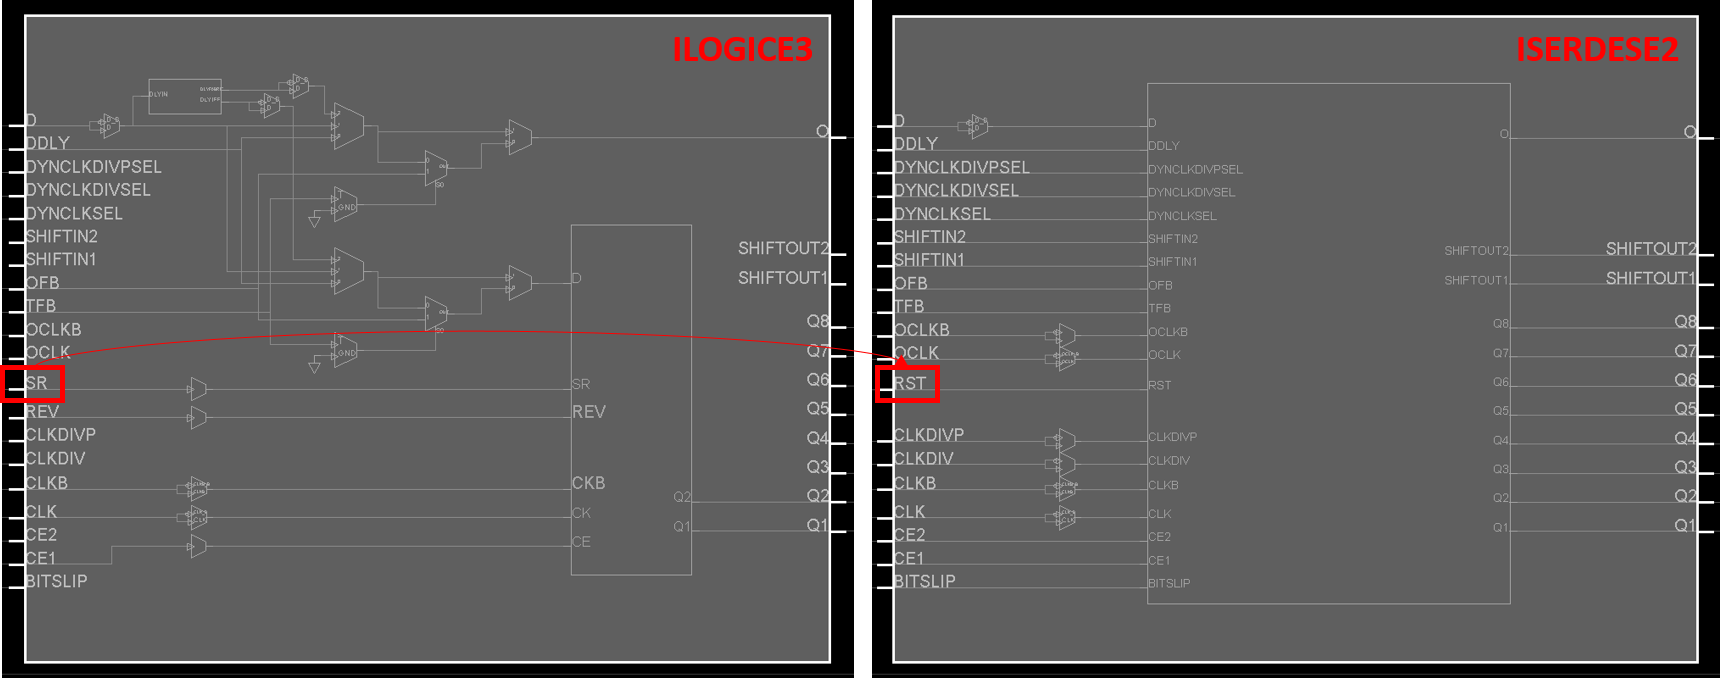
\includegraphics[width=.8\columnwidth]{pinRenaming.png}
        \caption{Pin renaming between an IDELAYE3 site (left) and ISERDESE2
        alternate site (right)}
        \label{fig:alternatePinRename}
      \end{figure}
      
      Unfortunatly these pin renamings cannot be automatically extracted from
      Vivado's Tcl interface, and so must be added manually. The XML example
      below shows how to add pin renamings to the Family Info.

\begin{lstlisting}[numbers=none]
      <name>ILOGICE3</name>
      <alternatives>
        <alternative>
          <name>ILOGICE2</name>
          |\textbf{<pinmaps>}|
          |\textbf{</pinmaps>}|
        </alternative>
        <alternative>
          <name>ISERDESE2</name>
          |\textbf{<pinmaps>}|
	        |\textbf{<pin>}|
	          |\textbf{<name>RST</name>}|
	          |\textbf{<map>SR</map>}|
	        |\textbf{</pin>}|
          |\textbf{</pinmaps>}|
        </alternative>
      </alternatives>
\end{lstlisting}
      
      \noindent A placeholder ``pinmaps'' tag is included for all alternate
      types in the initial family info file, all you need to do is fill in the pin
      mappings. To determine the actual pin mappings, you need to open two
      instances of the Vivado GUI. For each site in the Family Info, load the
      default type in one Vivado instance, load the the alternate type in the
      other instance, and visibly check what pins are renamed in the alternate
      type (as demonstrated in \autoref{fig:alternatePinRename}). You can be
      sure that pins are renamed if they connect to the same external tile
      wire. This process can be tedious, but there is currently no other
      solution. \autoref{tab:artix7PinMaps} shows the alternate types that
      require pin mappings for Artix7.
	  
	  \begin{table} [h!]
		\begin{center}
		\begin{tabu}{ |c|c| }
		\hline
		\textbf{Default Type} & \textbf{Alternate Type} \\
		\hline
		\hline 
		FIFO18E1 & RAMB18E1 \\
		\hline
		ILOGICE3 & ISERDESE2 \\
		\hline
		IOB33M & IPAD \\
		\hline
		IOB33S & IPAD \\
		\hline
		OLOGICE3 & OSERDESE2 \\
		\hline
		RAMBFIFO36E1 & FIFO36E1, RAMB36E1 \\
		\hline
		\end{tabu}
		\caption{Artix7 Alternate Types that require Family Info pin mappings}
		\label{tab:artix7PinMaps}
		\end{center}
      \end{table}
	  	  	  
	  \item The third hand edit is to remove invalid mux corrections. In some
	  cases, BELs might be incorrectly tagged as ``routing muxes'' or ``polarity
	  selectors'' even though they are not. This issue has mostly been fixed, but
	  it is still good practice to examine all of the mux corrections in the
	  Family Info and verify that they are correct.
	  
	  \item The final hand edit is to add missing compatible types. Some compatible
	  types can be automatically generated from Vivado, but not all. This means
	  that the missing compatible types must be added manually. The next section
	  (``Other Devices'') describes in more detail how to add compatible types to the Family Info.
	  	  
    \end{enumerate}
    
    \bigbreak \noindent
	\begin{large}
	\textbf{Other Devices}
	\end{large}
	  	
  	\noindent UltraScale and later devices require only one hand edit: adding 
  	missing compatible types (most compatible types can be determined
  	automatically). The XML listings below show the two compatible types that
  	were manually added in order to complete the Kintex UltraScale family info.

\begin{lstlisting}[numbers=none]
    <site_type>
      <name>SLICEL</name>
      <is_slice/>
      |\textbf{<compatible\_types>}|
        |\textbf{<compatible\_type>SLICEM</compatible\_type>}|
      |\textbf{</compatible\_types>}|
\end{lstlisting}  

\begin{lstlisting}[numbers=none]
    <site_type>
      <name>HRIO</name> 
      <is_iob/>
      |\textbf{<compatible\_types>}|
        |\textbf{<compatible\_type>HPIOB</compatible\_type>}|
      |\textbf{</compatible\_types>}|
\end{lstlisting} 
   
	\noindent For other device families, you may have to add additional compatible
	sites. It is up to you to determine what compatible sites need to be added
	through experimentation.
    	 
	\item Generate an XDLRC file from \texttt{Tincr} and RapidSmith2 device
	files using the steps shown in \autoref{sec:creatingNewSupportedDevices}.
	    
	\item Run the Family Builder in RapidSmith2. An example usage is shown below.

\begin{lstlisting}[numbers=none]
[ttown523@CB461-EE09968:�] java edu.byu.ece.rapidSmith.util.FamilyBuilders xc7a100tcsg324
\end{lstlisting}

	\noindent The Family Builder accepts one command line argument: a part name of
	a device in the family. Using the device files for the specified part, a Java
	file is created that contains all of the tile types and site types within
	the family. For example, the command above will generate a
	\texttt{edu.byu.ece.rapidSmith.device.families.Artix7.java} file which can
	be used to find site and tile types as follows:
    
\begin{lstlisting}[language=java,numbers=none]
SiteType siteType = Artix7.SiteTypes.SLICEL;
TileType tileType = Artix7.TileTypes.CLBLL_L;
\end{lstlisting}

	\noindent As you scroll through the newly created file, you will see the
	comment ``/* ------ CLASSIFICATIONS GO HERE ------ */''. Below the comment,
	tile and site classifications can be manually added to group similar types
	together. The classifications for Artix7 is shown below for reference.  

\begin{lstlisting}[language=java,numbers=none]
    /* ------ CLASSIFICATIONS GO HERE ------ */
        // Tile classifications
        _CLB_TILES.add(TileTypes.CLBLL_L);
        _CLB_TILES.add(TileTypes.CLBLL_R);
        _CLB_TILES.add(TileTypes.CLBLM_L);
        _CLB_TILES.add(TileTypes.CLBLM_R);

        _SWITCHBOX_TILES.add(TileTypes.INT_L);
        _SWITCHBOX_TILES.add(TileTypes.INT_R);

        _BRAM_TILES.add(TileTypes.BRAM_L);
        _BRAM_TILES.add(TileTypes.BRAM_R);
	
        _DSP_TILES.add(TileTypes.DSP_L);
        _DSP_TILES.add(TileTypes.DSP_R);
	
        _IO_TILES.add(TileTypes.LIOI3_TBYTESRC);
        _IO_TILES.add(TileTypes.LIOB33_SING);
        _IO_TILES.add(TileTypes.LIOI3_SING);
        _IO_TILES.add(TileTypes.LIOI3_TBYTETERM);
        _IO_TILES.add(TileTypes.LIOI3);
        _IO_TILES.add(TileTypes.LIOB33);
        _IO_TILES.add(TileTypes.RIOI3);
        _IO_TILES.add(TileTypes.RIOB33);
        _IO_TILES.add(TileTypes.RIOI3_SING);
        _IO_TILES.add(TileTypes.RIOI3_TBYTETERM);

		// Site classifications
        _SLICE_SITES.add(SiteTypes.SLICEL);
        _SLICE_SITES.add(SiteTypes.SLICEM);
	
        _BRAM_SITES.add(SiteTypes.RAMB18E1);
        _BRAM_SITES.add(SiteTypes.RAMB36E1);
        _BRAM_SITES.add(SiteTypes.RAMBFIFO36E1);

        _DSP_SITES.add(SiteTypes.DSP48E1);

        _IO_SITES.add(SiteTypes.IOB33);
        _IO_SITES.add(SiteTypes.IOB33S);
        _IO_SITES.add(SiteTypes.IOB33M);
        _IO_SITES.add(SiteTypes.IPAD);
        _IO_SITES.add(SiteTypes.OPAD);
\end{lstlisting}

\end{enumerate}


\noindent After these steps are complete, RapidSmith2 will have full support for
the generated family. This means that device files for any part within the
family can now be created.
 